\begin{center}
	\captionsetup{type = table}
	\begin{tblr}{ Q[l,m,3cm]  Q[l,m,6cm] }
		\textbf{Symbol} & \textbf{Bedeutung}\\ \hline[2pt]
		$|a|$ & Betrag, Länge eines Skalars \\ \hline
		$||\vec{a}||$ & Norm, Länge eines Vektors \\ \hline
		$\partial$ & partielle Ableitung \\ \hline
		$\subset,\supset$ & echte Teil-/Ober-menge\\ \hline
		$\subseteq, \supseteq$ & Teil-/Ober-menge \\\hline
		$\nabla$ & Nabla\\ \hline
		$\times$ & Kreuzprodukt \\ \hline
		$\text{sinh}(x)$ & $\frac{1}{2}\left(e^x -e^{-x} \right) = -i \cdot \text{sin} (i\cdot x)$\\ \hline
		$\text{cosh}(x)$ & $\frac{1}{2}\left(e^x +e^{-x} \right) = -i \cdot \text {cos} (i\cdot x)$\\ \hline
	\end{tblr}
	\caption{Allgemeine Symbole und Begriffe}\label{table:Test}
\end{center}

\textbf{skalares Feld:} eine Funktion, die jedem Punkt eines Raumes einen Skalar zuordnet. \\
\textbf{Vektor Feld:} eine Funktion, die jedem Punkt eines Raumes einen Vektor zuordnet. \\
\textbf{Definitionsbereich:} Bereich, für den eine Funktion definiert ist.\\
\textbf{Wertebereich:} Werte die die Funktion annehmen kann.\\
\textbf{Parameterdarstellung:} $C(t), C\in \mathbb{R}^3$ in Parameterdarstellung: $\gamma =
\begin{pmatrix}
	x(t)\\
	y(t)\\
	z(t)\\
\end{pmatrix}$\\

$\delta_{ij}$... Kronecker Delta
$\qquad \delta_{ij} =
   \left \{
   \begin{aligned}
	1,\ \text{falls}\qquad i=j\\
   0,\ \text{falls} \qquad i \neq j
	\end{aligned}
	\right .$\\

\subsection{Additionstheoreme:}\label{subs:Additionstheoreme}
$\sin(x)^2 + \cos(x)^2 = 1$\\

$\sin(x\pm y) = \sin(x)\cdot \cos(y) \pm \cos(x)\cdot \sin(y)$\\

$\cos(x\pm y) = \cos(x)\cdot \cos(y) \mp \sin(x)\cdot \sin(y)$\\


\subsection{Binomische Formeln und Binomischer Lehrsatz:}\label{subs:quadr_lösungsformel}
\begin{equation}
	x^2+px+q=0 \qquad x_{1/2}=-\frac{p}{2} \pm \sqrt{\left(\frac{p}{2}\right)^2-q}
\end{equation}\label{Quadratische Lösungsformel}

\begin{equation}
	{(a+b)}^n = \sum\limits_{k=0}^n \left ( \begin{matrix}
		n\\
		k\\
	\end{matrix} \right ) a^{n-k}\cdot b^k ,n \in \mathbb{N}
\end{equation}\label{eq:Binomischer_Lehrsatz}
\ \\



\subsection{Polynomdivision}
\begin{itemize}
	\item Polynom auf Form $x^3 + a\cdot x^2 + b \cdot x + c = 0$
	\item Nullstelle $x_1$ erraten. Eine gute Strategie ist, alle positiven
	und negativen Teiler des konstanten Terms durchzuprobieren.
	\item Polynom durch $(x-x_1)$ dividieren
\end{itemize}

Bsp.:\\

\captionsetup{type=figure}
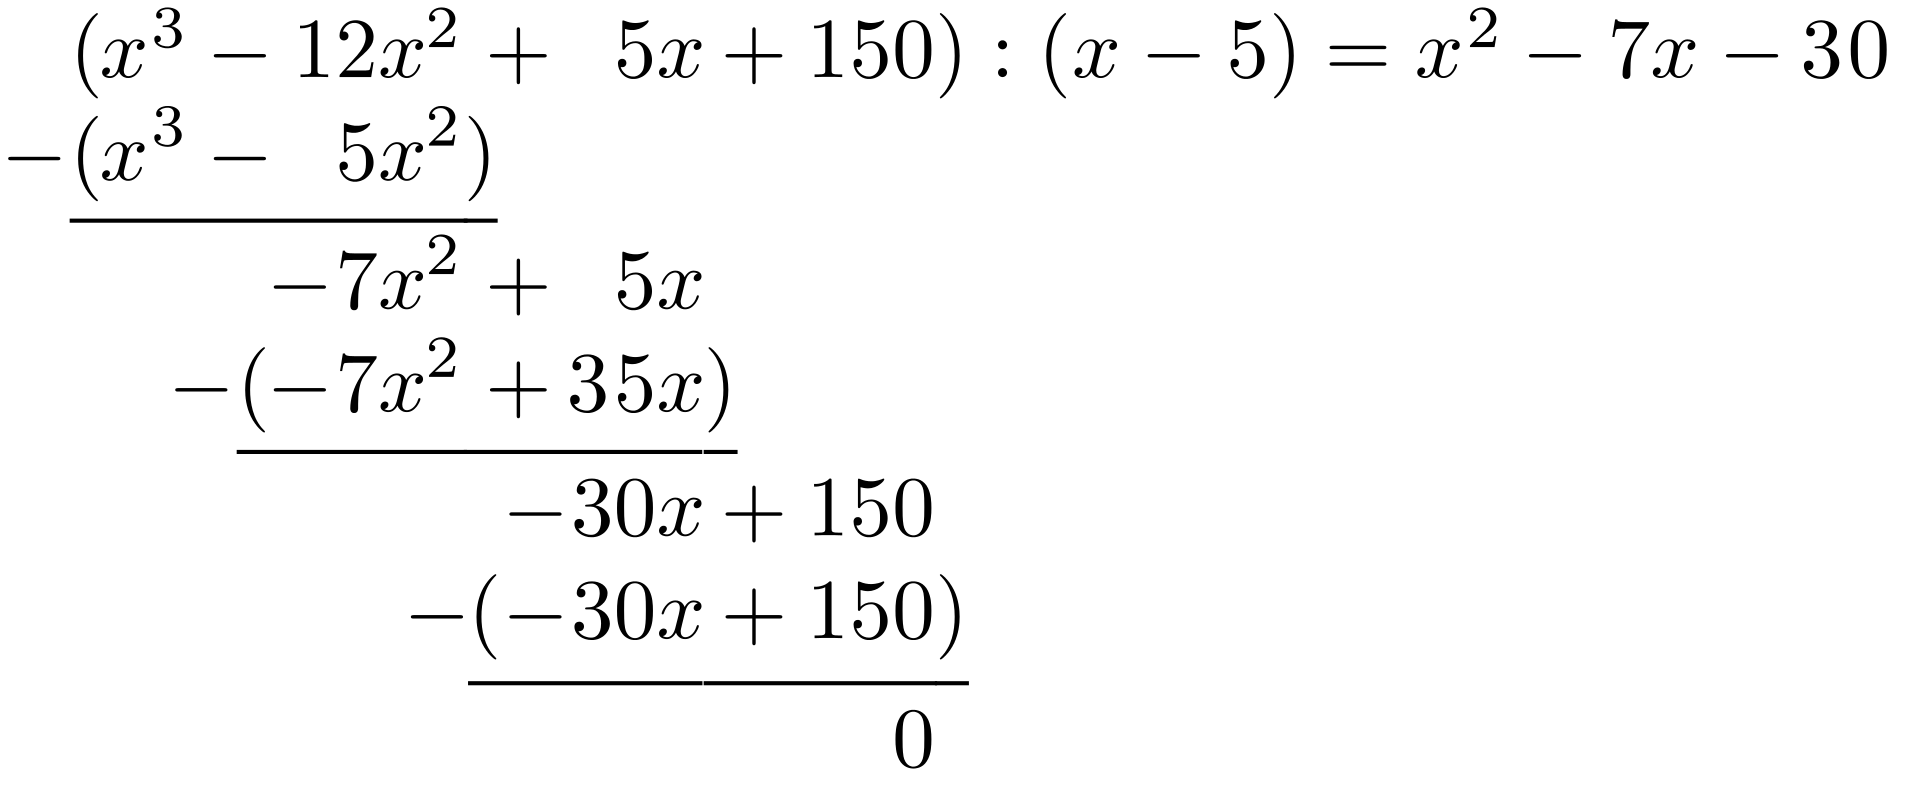
\includegraphics[width=0.6\textwidth]{../pictures/Polynomdivision.png}
\caption{Polynomdivision}\label{fig:Polynomdivision}

\subsection{Rechenregeln}
$x=\log_a(b) \Leftrightarrow a^x = b \qquad \log_e(x) = \ln(x)$\\
$\ln(a\cdot b) = \ln(a)+\ln(b) \qquad \ln\left( \frac{a}{b} \right) = \ln(a) - \ln(b) \qquad \ln(a^b)=b\cdot \ln(a) \qquad \log_a(a)=1 \qquad \log(1) = 0$\\

$(a\cdot b)^r = a^r \cdot b^r \qquad a^r\cdot a^s = a^{r+s} \qquad \frac{a^r}{a^s}=a^{r-s} \qquad \sqrt[r]{a} = a^{\frac{1}{r}}$\\
$(a^r)^s =a^{r\cdot s} \qquad \sqrt[s]{a^r} = a^{\frac{r}{s}}$\\


\subsection{Identitäten}\label{subs:Identitäten}
\textbf{Ableitung/Umkehrfunktion:} $(f^{-1}(y))'=\frac{1}{f'(f^{-1}(y))}$